%%%%%%%%%%%%%%%%%%%%%%%%%%%%%%%%%%%%%%%%%%%%%%%%%%%%%%%%%%%%%%%%%%%%%
%
%  This is a sample LaTeX input file for your contribution to 
%  the MC2013 conference. Modified by R.C. Martineau at INL from A. 
%  Sood at LANL, from J. Wagner ORNL who obtained the original class 
%  file by Jim Warsa, LANL, 16 July 2002}
%
%  Please use it as a template for your full paper 
%    Accompanying/related file(s) include: 
%       1. Document class/format file: mc2013.cls
%       2. Sample Postscript Figure:   figure.eps
%       3. A PDF file showing the desired appearance: template.pdf 
%    Direct questions about these files to: richard.martinea@inl.gov
%
%    Notes: 
%      (1) You can use the "dvips" utility to convert .dvi 
%          files to PostScript.  Then, use either Acrobat 
%          Distiller or "ps2pdf" to convert to PDF format. 
%      (2) Different versions of LaTeX have been observed to 
%          shift the page down, causing improper margins.
%          If this occurs, adjust the "topmargin" value in the
%          mc2013.cls file to achieve the proper margins. 
%
%%%%%%%%%%%%%%%%%%%%%%%%%%%%%%%%%%%%%%%%%%%%%%%%%%%%%%%%%%%%%%%%%%%%%


%%%%%%%%%%%%%%%%%%%%%%%%%%%%%%%%%%%%%%%%%%%%%%%%%%%%%%%%%%%%%%%%%%%%%
\documentclass{mc2013}
%
%  various packages that you may wish to activate for usage 
\usepackage{graphicx}
\usepackage{tabls}
\usepackage{afterpage}
\usepackage{cites}
\usepackage{amsmath}
\usepackage{amssymb}
\usepackage{listings}
\usepackage{float}
\usepackage{caption}
\usepackage{subcaption}
\usepackage{verbatim}


\usepackage{tgheros}
\usepackage{xcolor}
\lstset { 
    basicstyle=\sffamily
    breaklines=true
    language=C++,
    backgroundcolor=\color{black!5}, % set backgroundcolor
    basicstyle=\footnotesize,% basic font setting
    columns = flexible
}

%\usepackage{epsf}
%
%
% Insert authors' names and short version of title in lines below
%
\newcommand{\authorHead}      % Author's names here
   {A. Alfonsi, C. Rabiti, D. Mandelli, J.J. Cogliati, R.A. Kinoshita}  
\newcommand{\shortTitle}      % Short title here
   {RAVEN as a tool for Dynamic Probabilistic Risk Assessment: Software Overview}  
%%%%%%%%%%%%%%%%%%%%%%%%%%%%%%%%%%%%%%%%%%%%%%%%%%%%%%%%%%%%%%%%%%%%%
%
%   BEGIN DOCUMENT
%
%%%%%%%%%%%%%%%%%%%%%%%%%%%%%%%%%%%%%%%%%%%%%%%%%%%%%%%%%%%%%%%%%%%%%
\begin{document}

%
%      Headers and Footers
\afterpage{%
\fancyhf{}%
\fancyhead[CE]{              
{\scriptsize \authorHead}}                                                
\fancyhead[CO]{               
{\scriptsize \shortTitle}}                  
%\lfoot{\scriptsize{
%ANS PSA 2013 International Topical Meeting  on Probabilistic Safety Assessment and Analysis
%Columbia, SC, September  22-26, 2013, on CD-ROM, American Nuclear Society, LaGrange Park, IL (2013), 
%\\ Sun Valley, Idaho, USA, May 5-9, 2013.}}%
\rfoot{\thepage/\totalpages{}}%

\pagestyle{fancy}
%\setlength{\topmargin}{-20pt}
}
 
\normalsize

%\setlength{\baselineskip}{16.8pt}
\vspace{-3pt}

% 
% TITLE
%

\begin{center}
\textbf{\large \\%
Dynamic Event Tree Analysis Through RAVEN
}
% 
% FIRST AUTHORS 
%


\setlength{\baselineskip}{14pt}
\textbf{A. Alfonsi*, C. Rabiti*, D. Mandelli*, J.J. Cogliati*, R.A. Kinoshita*, A. Naviglio$^{\dag}$} \\ %\footnote{Footnote, if necessary, in Times New Roman font and font size 9} 
\vspace{3 mm}
* Idaho National Laboratory \\
2525 Fremont Avenue, Idaho Falls, ID 83415 \\
\{andrea.alfonsi, cristian.rabiti, diego.mandelli, joshua.cogliati, robert.kinoshita\}@inl.gov \\
\vspace{3 mm}
$^{\dag}$ Universit\`a di Roma ``La Sapienza'', Dipartimento Ingegneria Energetica e Nucleare  \\
Via Eudossiana, 18, 00184, Rome, Italy \\
antonio.naviglio@uniroma1.it

\end{center}

%
% SET RAGGED RIGHT MARGIN
%
%\raggedright


\section*{ABSTRACT} 
\begin{quote}
\begin{small}
Conventional \textbf{E}vent-\textbf{T}ree (\textbf{ET}) based methodologies are extensively used as tools to perform reliability and safety assessment of complex and critical engineering systems. 
One of the disadvantages of these methods is that timing/sequencing of events and system dynamics is not explicitly accounted for in the analysis.
In order to overcome these limitations several techniques, also know as \textbf{D}ynamic \textbf{P}robabilistic \textbf{R}isk \textbf{A}ssessment (\textbf{D-PRA}), have been developed. \textbf{M}onte-\textbf{C}arlo (MC) and \textbf{D}ynamic \textbf{E}vent \textbf{T}ree (\textbf{DET}) are two of the most widely used D-PRA methodologies to perform safety assessment of \textbf{N}uclear \textbf{P}ower \textbf{P}lants (NPP).
In the past two years, the Idaho National Laboratory (INL) has developed its own tool to perform Dynamic PRA: \textbf{RAVEN} (\textbf{R}eactor \textbf{A}nalysis and \textbf{V}irtual control \textbf{EN}vironment).
RAVEN has been designed in a high modular and pluggable way in order to enable easy integration of different programming languages (i.e., C++, Python) and coupling with other application including the ones based on the MOOSE framework, developed by INL as well.
RAVEN performs two main tasks: 1) control logic driver for the new Thermo-Hydraulic code RELAP-7 and 2) post-processing tool.
In the first task, RAVEN acts as a deterministic controller in which the set of control logic laws (user defined) monitors the RELAP-7 simulation and controls the activation of specific systems.
Moreover, RAVEN also models stochastic events, such as components failures, and performs uncertainty quantification. Such stochastic modeling is employed by using both MC and DET algorithms.
In the second task, RAVEN processes the large amount of data generated by RELAP-7 using data-mining based algorithms.
This paper focuses on the first task and shows how it is possible to perform the analysis of dynamic stochastic systems using the newly developed RAVEN DET capability.
As an example, the Dynamic PRA analysis, using Dynamic Event Tree, of a simplified pressurized water reactor for a Station Black-Out scenario is presented.

\emph{Key Words}: Reactor Simulation, Probabilistic Risk Assessment, PRA, Dynamic Event Tree, RELAP-7 %, Three Miles Island, 
\end{small} 
\end{quote}

\setlength{\baselineskip}{14pt}
\normalsize

%%%%%%%%%%%%%%%%%%%
\Section{INTRODUCTION} 
%%%%%%%%%%%%%%%%%%%
RAVEN (\textbf{R}eactor \textbf{A}nalysis and \textbf{V}irtual control \textbf{EN}viroment)~\cite{ravenFY12,mandelliANS2012} is a software tool that acts as the control logic driver for the newly developed Thermal-Hydraulic code RELAP-7  (\textbf{R}eactor \textbf{E}xcursion and \textbf{L}eak \textbf{A}nalysis \textbf{P}rogram). The goal of this paper is to highlight the newly developed  Dynamic Event Tree module embedded in the code and its utilization in conjunction with RELAP-7. RAVEN is a multi-purpose \textbf{P}robabilistic \textbf{R}isk \textbf{A}ssessment (PRA) software framework that allows dispatching different functionalities. 
It is designed to derive and actuate the control logic required to simulate the plant control system and operator actions (guided procedures) and to perform both Monte-Carlo sampling of random distributed events and Event Tree based analysis. 
In order to facilitate the input/output handling, a \textbf{G}raphical \textbf{U}ser \textbf{I}nterface (GUI) and a post-processing data mining module, based on dimensionality and cardinality reduction, are available.
This paper wants to provide an overview of the DET structure, highlighting the mathematical framework from which its structure is derived, the main conceptual decisions have been taken and its software layout. In addiction it will be shown a \textbf{S}tation \textbf{B}lack \textbf{O}ut (SBO) Dynamic Event Tree based analysis of a simplified \textbf{P}ressurized \textbf{W}ater \textbf{R}eactor (PWR) model.
\vspace{-5mm}
%%%%%%%%%%%%%%%%%%%%%%%%%%%%%%
\Section{RAVEN OVERVIEW} 
%%%%%%%%%%%%%%%%%%%%%%%%%%%%%%
\Subsection{Mathematical Framework}
\label{sec:mathFramework}
Let be $\bar{\theta}(t)$ a vector describing the plant status in the phase space; the dynamic of the plant, including the control system, can be summarized by the following equation:
\begin{equation}
\frac{\partial \bar{\theta}}{\partial t} = \bar{H}(\theta(t),t)
\label{eq:SystemDynamics}
\end{equation}
In the above equation it is assumed the time differentiability in the phase space. Performing an arbitrary decomposition of the phase space, the following statement is obtained:
\begin{equation}
\bar{\theta}=\binom{\bar{x}}{\bar{v}}
\label{eq:firstDecomposition}
\end{equation}
The decomposition is made in such a way that $\bar{x}$ represents the unknowns solved by RELAP-7, while $\bar{v}$ are the variables directly controlled by the control system (i.e., RAVEN). Equation~\ref{eq:SystemDynamics} can now be rewritten as follows:
\begin{equation}
\begin{cases} 
\dfrac{\partial \bar{x}}{\partial t} = \bar{F}(\bar{x},\bar{v},t) \\ 
\dfrac{\partial \bar{v}}{\partial t} = \bar{V}(\bar{x},\bar{v},t) \\
\end{cases}
\label{eq:generalSystemEquation}
\end{equation}
It is possible to note that the function $\bar{V}(\bar{x},\bar{v},t)$ representing the control system, does not depend on the knowledge of the complete status of the system but on a restricted subset (i.e. control variables) $\bar{C}$:
\begin{equation}
\begin{cases} 
\dfrac{\partial \bar{x}}{\partial t} = \bar{F}(\bar{x},\bar{v},t) \\
\bar{C} = \bar{G}(\bar{x},t) \\ 
\dfrac{\partial \bar{v}}{\partial t} = \bar{V}(\bar{x},\bar{v},t) 
\end{cases}
\label{eq:generalSystemEquationwithControl}
\end{equation}
The system of equations in Eq.~\ref{eq:generalSystemEquationwithControl} is fully coupled and has commonly been solved by an operator splitting approach. The reasons for this choice are several:
\begin{itemize}
\item Control system reacts with an intrinsic delay
\item The reaction of the control system might move the system between two different discrete states and
therefore numerical errors will be always of first order unless the discontinuity is treated explicitly.
\end{itemize}
Thus, RAVEN is using this approach to solve Eq.~\ref{eq:generalSystemEquationwithControl} which becomes:
\begin{equation}
\begin{cases} 
\dfrac{\partial \bar{x}}{\partial t} = \bar{F}(\bar{x},\bar{v}_{t_{i-1}},t) \\
\bar{C} = \bar{G}(\bar{x},t) & t_{i-1}\leq t\leq t_{i} = t_{i-1} + \Delta t_{i}\\ 
\dfrac{\partial \bar{v}}{\partial t} = \bar{V}(\bar{x},\bar{v}_{t_{i-1}},t) \\
\end{cases}
\label{eq:generalSystemEquationwithControlSplitting}
\end{equation}
Even if all information needed is contained in $\bar{x}$ and $\bar{v}$, it is not a practical and efficient way to implement the control system. Hence, a system of auxiliary variables has been introduced.
The auxiliary variables are those that in statistical analysis are artificially added, when possible, to non-Markovian systems into the space phase to obtain a Markovian behavior back, so that only the information of the previous time step is needed to determine the future status of the system.
Thus, the introduction of the auxiliary system into the mathematical framework leads to the following formulation of the Eq.~\ref{eq:generalSystemEquationwithControlSplitting}:
\vspace{-2mm}
\begin{equation}
\begin{cases} 
\dfrac{\partial \bar{x}}{\partial t} = \bar{F}(\bar{x},\bar{v}_{t_{i-1}},t) \\
\bar{C} = \bar{G}(\bar{x},t) & t_{i-1}\leq t\leq t_{i} = t_{i-1} + \Delta t_{i}\\ 
\dfrac{\partial \bar{a}}{\partial t} = \bar{A}(\bar{x},\bar{C},\bar{a}_{t_{i-1}},\bar{v}_{t_{i-1}},t) \\
\dfrac{\partial \bar{v}}{\partial t} = \bar{V}(\bar{x},\bar{C},\bar{v}_{t_{i-1}},\bar{a},t) 
\end{cases}
\label{eq:generalSystemEquationwithControlSplittingAndAux}
\end{equation}
\Subsection{Software Overview}
RAVEN, is plugged with the software environment MOOSE~\cite{MOOSE}. MOOSE is a computer simulation framework,  developed at Idaho National Laboratory (INL), that simplifies the process for predicting the behavior of complex systems and developing non-linear, multi-physics simulation tools. Other than providing the algorithms for the solution of the differential equation, MOOSE also provides all the manipulation tools for the \verb!C++! classes containing the solution vector. This framework has been used to construct and develop the Thermal-Hydraulic code RELAP-7, giving an enormous flexibility in the coupling procedure with RAVEN. 
RELAP-7 is the next generation nuclear reactor system safety analysis. It will become the main reactor systems simulation toolkit for RISMC (\textbf{R}isk \textbf{I}nformed \textbf{S}afety \textbf{M}argin \textbf{C}haracterization)~\cite{mandelliANS_RISMC} project and the next generation tool in the RELAP reactor safety/systems analysis application series. 
RAVEN has been developed in a high modular and pluggable way in order to enable easy integration of different programming languages (i.e., \verb!C++!, \verb!Python!) and coupling with other applications including the ones based on MOOSE. The code consists of four main modules:
\vspace{-5mm}
\begin{itemize}
\itemsep0em
\item RAVEN/RELAP-7 interface
\item Python Control Logic 
\item External Python Manager
\item Graphical User Interface 
\end{itemize}
\vspace{-5mm}
The RAVEN/RELAP-7 interface, coded in \verb!C++!, is the container of all the tools needed to interact with RELAP-7/MOOSE. It has been designed in order to be general and pluggable with different solvers simultaneously in order to allow an easier and faster development of the control logic/PRA capabilities for multi-physics applications.
The interface provides all the capabilities to generate the monitored quantities and accordingly modify the controlled parameters in the RELAP-7/MOOSE calculation.
\\The control logic module is used to drive a RAVEN/RELAP-7 calculation. Up to now it is implemented by the user via \verb!Python! scripting. The reason of this choice is to try to preserve generality of the approach in the initial phases of the project so that further specialization is possible and  inexpensive. The implementation of the control logic via \verb!Python! is rather convenient and flexible. The user only needs to know few \verb!Python! syntax rules in order to build an input. Although this extreme simplicity, it will be part of the GUI task to automatize the construction of the control logic scripting in order to minimize user effort. 
\\The core of PRA analysis is contained in an external driver/manager. It consists in a Python framework that contains the capabilities and interfaces to drive a PRA analysis. Its basic infrastructure in connection with the Dynamic Event Tree module will be discussed in section~\ref{sec:CPUInfrastructure}   
\\As previously mentioned, a Graphical User Interface (GUI) is not required to run RAVEN, but it represents an added value to the whole code. The GUI is compatible with all the capabilities actually present in RAVEN.  Its development is performed using QtPy, which is a \verb!Python! interface for a \verb!C++! based library (\verb!C++!) for GUI implementation. The GUI is based on a software named Peacock, which is a GUI interface for MOOSE based application and, in its base implementation, is only able to assist the user in the creation of the input.  In order to make it fit all the RAVEN needs, the GUI has been specialized and is in continuous evolution.
\vspace{-5mm}
%%%%%%%%%%%%%%%%%%%%%%%%%%%%
\Section{THE DYNAMIC EVEN TREE METHODOLOGY}
%%%%%%%%%%%%%%%%%%%%%%%%%%%%
\label{sec:DET_methodology}
In technological complex systems, as nuclear power  plants, an accident scenario begins with an initiating event and, through the interaction of dynamics and stochastics, evolves over time. This mutual action leads to the production of infinitely many different scenarios, that define a continuous dynamic event tree with infinite branches. At each time point, the stochastic variability of the accident outcomes is determined by a multi-variate probability distribution.
The PRA analysis needs an approximation to this distribution for selected consequence variables. 
A way to achieve this goal is an Event Tree approach. In dynamic PRA analysis, Conventional Event Tree (ET) sequences are run simultaneously starting from a single initiating event. The branchings occur at user specified times and/or when an action is required by the operator and/or the system, creating a deterministic sequence of events based on the time of their occurrence. 
\begin{figure}[h] 
  \centering
     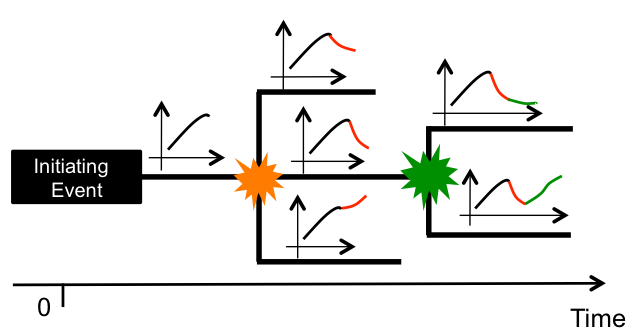
\includegraphics[width=0.8\textwidth]{figures/DET_schemeFlow.png}
  \caption{Dynamic Event Tree Conceptual Scheme.}
   \label{fig:DET_schemeFlow}
\end{figure}
\\One of the disadvantages of this method is that timing/sequencing of events and system dynamics is not explicitly accounted for in the analysis.In order to overcome these limitations a ``dynamic'' approach is needed. The Dynamic Event Tree (DET) technique brings several advantages, among which the fact that it simulates probabilistic system evolution in a way that is consistent with the severe accident model. This leads to a more realistic and mechanistically consistent analysis of the system taken in consideration. The dynamic PRA, in general, and the Dynamic Event Tree methodologies, in particular, are designed to take the timing of events explicitly into account which can become very important especially when uncertainties in complex phenomena are considered. Hence, the main idea of this methodology is to let a system code (i.e. RELAP-7) determine the pathway of an accident scenario within a probabilistic ``environment''. \\ Figure~\ref{fig:DET_schemeFlow} schematically shows the DET logic. As already mentioned, the accident sequence starts with an initiating event. Based on an user defined branching logic, driven by \textbf{P}robabilistic \textbf{D}istribution \textbf{F}unctions (PDFs), an event occurs at a certain time $t=T$. The simulation spoons $n$ different branches. In each of them, the branching event determines a different consequence (carrying on associated probabilities). Each sequence continues until another event occurs and a new set of branching is spooned. The simulation ends when an exit condition or a maximum mission time is reached.    
%%%%%%%%%%%%%%%%%%%%%%%%%%%%%%
\Section{RAVEN APPROACHING DYNAMIC METHODOLOGIES: ANDREA MODULE} 
%%%%%%%%%%%%%%%%%%%%%%%%%%%%%%
\label{sec:DETRavenApproach}
RAVEN is now able to perform Dynamic Event Tree analysis through the newly developed module "\textbf{AN}alysis of \textbf{D}ynamic \textbf{RE}actor \textbf{A}ccident evolution" (ANDREA), that has been included in the RAVEN external Python manager. Following the philosophy of the DET approach, this module lets RELAP-7 find the path of an accident sequence, in a probabilistic point of view. When the system achieves certain conditions that would lead to alternative accident ways (i.e. an event occurs), a sampler generates a new set of branches (new possible scenarios), associating for each a conditional probability.  
As easily understandable, in complex cases, the number of branches may become extremely big. In order to avoid unacceptable growth of problem due by an excessive number of branches, the user needs to specify an exit logic (termination laws), for example maximum mission time, rules based on the simulator physic model (i.e. Maximum temperature of the fuel cladding, etc.), and/or probabilistic thresholds. In other similar codes, one of the most common termination law is a probability cut-off: a branch execution is truncated when its probability falls below a given limit. No countermeasures are generally taken to conserve the global probability. This approach may introduce a big impact on the probability of key events, if the user defined limit is not small enough that the influence on the final branch probability is not negligible.  In order to avoid these issues and preserve the probability conservation, the user can not directly input a branching probability cut-off. 
\\ As can be inferred from the previous dissertation, the package is aimed to provide capabilities to:
\vspace{-5mm}
\begin{itemize}
\itemsep0em
\item explore possible pathways through which the system can evolve
\item quantify the probability of these scenarios
\end{itemize}
\vspace{-5mm}
These main tasks are accomplished based on user specified branching and termination rules, model of the system in RELAP-7, probability assignment rules to accident sequences (either by inputed values or/and by distribution functions).
Regarding the branching rules,  

 
%%%%%%%%%%%%%%%%%%%%%%%%%%%%%%
\Subsection{Computational Infrastructure} 
\label{sec:CPUInfrastructure}
%%%%%%%%%%%%%%%%%%%%%%%%%%%%%%


%%%%%%%%%%%%%%%%%%%%%%%%%%%%%%
\Section{SOFTWARE LAYOUT AND CALCULATION FLOW} 
\label{sec:swLayoutCalcFlow}
%%%%%%%%%%%%%%%%%%%%%%%%%%%%%%
to add
%%%%%%%%%%%%%%%%%%%%%%%%
\Section{DEMO FOR A PWR PRA ANALYSIS} 
%%%%%%%%%%%%%%%%%%%%%%%%
to add 
%%%%%%%%%%%%%%%%%%%%%%%%%%%%%%
\Subsection{Station Black Out (SBO) analysis} 
%%%%%%%%%%%%%%%%%%%%%%%%%%%%%%
to add
%%%%%%%%%%%%%%%%%%%%%%%%%%%%%%
\Subsection{Results} 
%%%%%%%%%%%%%%%%%%%%%%%%%%%%%%
to add
%%%%%%%%%%%%%%%%%
\section{CONCLUSIONS AND FUTURE WORK}
%%%%%%%%%%%%%%%%%
to add
%%%%%%%%%%%%%%%%%%%%%%%%%%%%%%%%%%%%%%%%%%%%%%%%%%%%%%%%%%%%%%%%%%%%%%%%%%%%%%%%
\section*{ACKNOWLEDGMENT}
%%%%%%%%%%%%%%%%%%%%%%%%%%%%%%%%%%%%%%%%%%%%%%%%%%%%%%%%%%%%%%%%%%%%%%%%%%%%%%%%
This work is supported by the U.S. Department of Energy, under DOE Idaho Operations Office Contract DE-AC07-05ID14517. Accordingly, the U.S. Government retains a nonexclusive, royalty-free license to publish or reproduce the published form of this contribution, or allow others to do so, for U.S. Government purposes.

\bibliographystyle{ieeetr}
\bibliography{bibl}


\end{document}


